%\documentclass[hyperref={pdfpagelabels=false}]{beamer}
\documentclass{beamer}
\usepackage{textcomp}
\usepackage[german]{babel}
\usepackage[utf8]{inputenc}
\usepackage{times}
\usepackage[T1]{fontenc}

%gets rid of navigation symbols
\setbeamertemplate{navigation symbols}{}

\mode<presentation>
{
  \usetheme{Marburg}
  \setbeamercovered{transparent}
}

\title {Networked Embedded Systems VU}
\subtitle {LightBus}
\author{R. Annessi,\\ A. Heinisch,\\ N. Mayerhofer}

% custom date
\usepackage{datetime}
\newdateformat{customdate}{\monthname{ }\THEYEAR}
\date{\customdate\today}


\logo{

\includegraphics[height=0.5cm]{./images/logo_neu.jpg}
}


\begin{document}
\begin{frame}
  \titlepage
\end{frame}
% logo only on title page
 \logo{}

\begin{frame}{Table of Contents}
  \tableofcontents
\end{frame}


\section{Project Outline}
\begin{frame}{Defining project goals}%{}
\begin{center}
\begin{itemize}
  \item embedded communication for home automation are expensive
    \begin{itemize}
      \item certification necessary
      \item licence needed
      \item ...
    \end{itemize}
  \item implementation of given protocols are often heavily
  \item migration of additional components in given systems claims expertise
\end{itemize}
\end{center}
\end{frame}

\begin{frame}{Project goals}%{}
\begin{center}
\begin{itemize}
 \item \begin{large}building a fault tolerant bus protocol\end{large}
 \item \begin{large}separation of communication and application layers\end{large}
 \item \begin{large}providing basic fault tolerance\end{large}
 \item \begin{large}easy adaptable to existing projects\end{large}
 \item \begin{large}easy migrateable to existing systems\end{large}
\end{itemize}
\end{center}
\end{frame}

\begin{frame}{Group subject}{Synchronous Clocks}
  \begin{itemize}
    \item \begin{large}comparison of clock sync algorithms\end{large}
    \item \begin{large}implementation of an algorithm including\end{large}
      \begin{itemize}
	\item time estimation
	\item feasibility estimation
      \end{itemize}
    \item \begin{large}testing under fault conditions\end{large}
  \end{itemize}
\end{frame}

\section{Bus Protocol}
\begin{frame}{Bus protocol}{ULFTRTP}
\begin{center}
%\includegraphics[width=0.9\textwidth]{../images/presentation/brainwaves.png}
\begin{itemize}
  \item \begin{large}balanced bus tailored to our needs\end{large}
  \item \begin{large}csma/ca\end{large}
 \item \begin{large}non starvation handling\end{large}
 \item \begin{large}source/destination addressing\end{large}
\end{itemize}
\end{center}
\end{frame}

\begin{frame}{}%{}
\begin{center}
%\includegraphics[width=0.9\textwidth]{../images/presentation/brainwaves.png}
\begin{itemize}
  \item \begin{large}\end{large}
 \item \begin{large}\end{large}
 \item \begin{large}\end{large}
 \item \begin{large}\end{large}
\end{itemize}
\end{center}
\end{frame}


%welche gibts?
%vergleichen
%welche kommen in Frage
\section{Clock Synchronisation}
\begin{frame}{Problems caused by clock synchronisation}%{}
\begin{center}
%\includegraphics[width=0.9\textwidth]{../images/presentation/brainwaves.png}
\begin{itemize}
  \item \begin{large}assumption of timebase\end{large}
 \item \begin{large}synchronisation clock vs. message\end{large}
 \item \begin{large}adjustment method\end{large}
 \item \begin{large}latency correction\end{large}
\end{itemize}
\end{center}
\end{frame}


\begin{frame}{Clock Synchronisation}{clocks \& methodes}
  \begin{center}
  %\includegraphics[width=0.9\textwidth]{../images/presentation/brainwaves.png}
  \begin{itemize}
    \item \begin{large}clock positioning\end{large}
    \begin{itemize}
      \item centralized
      \item distributed
    \end{itemize}
    \item \begin{large}distributed clock algorithms\end{large}
    \begin{itemize}
      \item precision time protocol
      \item reference broadcast synchronization
    \end{itemize}
  \item \begin{large}Methode we used\end{large}
  \end{itemize}
  \end{center}
\end{frame}


\section{Time Plan}
\begin{frame}{Time Plan}
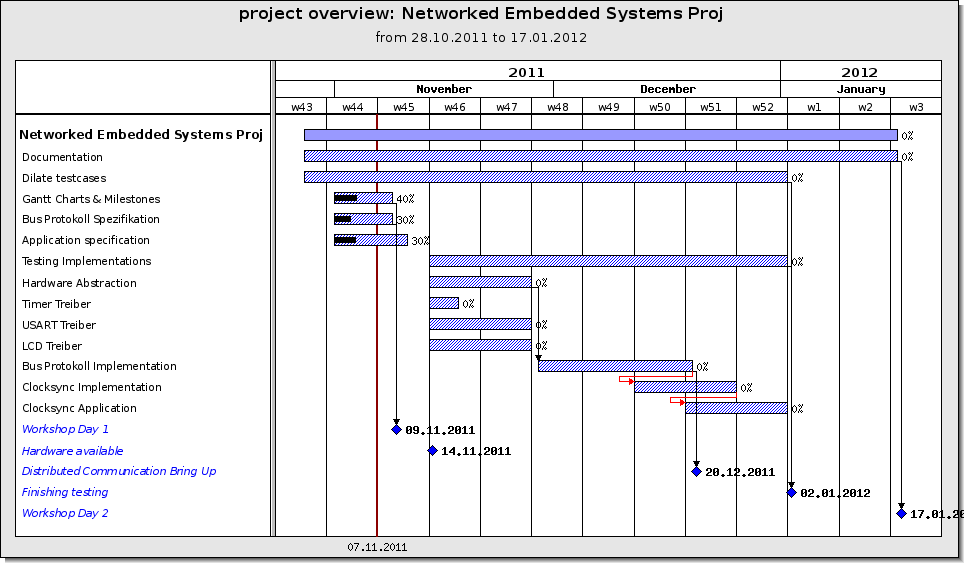
\includegraphics[width=1.0\textwidth]{./images/201111_ganttchart.png}
\vspace{1cm}
\end{frame}

\begin{frame}
\begin{center}
\begin{Huge}\textbf{Thank you!}\end{Huge}
\end{center}
\end{frame}


\begin{frame}{Questions}
\begin{center}

\includegraphics[width=0.7\textwidth]{./images/question-marks.png}
\end{center}
\end{frame}


\end{document}